\documentclass[12pt]{article}
\usepackage{amsmath}
\usepackage{listings}
\usepackage{xcolor}
\usepackage{float}
\usepackage{url}

\definecolor{codegreen}{rgb}{0,0.6,0}
\definecolor{codegray}{RGB}{4,118,219}
\definecolor{codepurple}{rgb}{0.58,0,0.82}
\definecolor{backcolour}{RGB}{0,27,51}
\definecolor{textcolour}{RGB}{38, 149, 245}

\lstdefinestyle{mystyle}{
    backgroundcolor=\color{backcolour},   
    commentstyle=\color{codegreen},
    keywordstyle=\color{magenta},
    numberstyle=\tiny\color{codegray},
    stringstyle=\color{codepurple},
    basicstyle=\ttfamily\color{textcolour}\footnotesize,
    breakatwhitespace=false,         
    breaklines=true,                 
    captionpos=b,                    
    keepspaces=false,                 
    numbers=left,                    
    numbersep=5pt,                  
    showspaces=false,                
    showstringspaces=false,
    showtabs=false,                  
    tabsize=2
}

\usepackage{setspace}
\onehalfspacing
%\doublespacing

\lstset{literate=%
    {Ö}{{\"O}}1
    {Ä}{{\"A}}1
    {Ü}{{\"U}}1
    {ß}{{\ss}}1
    {ü}{{\"u}}1
    {ä}{{\"a}}1
    {ö}{{\"o}}1
    {~}{{\textasciitilde}}1
}

\lstset{style=mystyle}

    \title{\textbf{Bachelorarbeit}}
    \author{Jan Philipp Fortowski}
    \date{xx.xx.2024}
    
    \addtolength{\topmargin}{-3cm}
    \addtolength{\textheight}{3cm}
\usepackage{graphicx}
\begin{document}


\maketitle
\cleardoublepage
% \phantomsection
\tableofcontents
\cleardoublepage
% \phantomsection
\thispagestyle{empty}



\section{Fully Connected Layer / Feed Forward Layer}
In diesem Kapitel werden die Fully Connected Layer betrachtet, welche genau so aufgebaut sind, wie bei den Feed Forward Networks. genau genommen wird im Prinzip einfach ein Feed Forward network am Ende des Convolutional networks eingesetzt, denn die Fully Connected layer werden nur am Ende benutzt. Wenn in einem netzwerk nur die Fully Connected Layer verwendet werden, dann handelt es sich um ein Feed Forward Network. 
Das Grundprinzip ist vergleichbar kompliziert. Jede Schicht enthält sogenannte Knoten. Diese knoten sind mit den Neuronen in einem Gehirn vergleichbar.

TODO Bild von Neuronen und Activations/Knoten

Alle Knoten einer Schicht, sind mit allen Knoten der nächsten Schicht verbunden. Diese Verbindungen werden gewichtet, also müssen Gewichte gespeichert werden, die festlegen, wie wichtig der Input eines jeweiligen Knotens für den Aktuellen Knoten ist. Diese Knoten können angepasst werden, das heißt, dass kleine inkrementelle Anpassungen mit jeder Lern-Iteration vorgenommen werden, um das Netzwerk Stück für Stück einem Fehler-Minimum anzupassen. 

TODO Bild von einem Neuronalen netzwerk mit allen verbindungen

Besonders für Lineare Problemen, die nicht durch den Nullpunkt eines Koordinatensystems gehen ist es Notwendig, auch Biases mit einzurechnen. Für die Bild Erkennung ist das normalerweise nicht wichtig, und da sich die Convolutions auf die Bilderkennung Spezialisieren, wird es für dieses Projekt nicht notwendig sein, Biases einzuplanen.

In diesem Kapitel werden nun zunächst der generelle Aufbau der Klasse "FullyConnectedLayer" dargelegt, und in den beiden Unterkapiteln wird dann speziell auf den ForwardPass und auf die Backpropagation eingegangen, zusammen mit den Mathematischen Grundlagen und dem dazugehörigen Code.

Zunächst muss die Klasse erstellt werden. Die Objektvariablen sind diese:
    
\begin{lstlisting}[language=Java]
public class FullyConnectedLayer extends Layer {
    double[][] weights;
    int inLength;
    int outLength;
    double learnRate;

    private double[] lastZ;
    private double[] lastInput;
\end{lstlisting} 
in den "weights" werden die Gewichte gespeichert zwischen den Inputs und den Knoten der Schicht. Diese können angepasst werden, um den Fehler des Netzwerkes zu minimieren, damit es korrekte Klassifizierungen vornehmen kann.
Mit "inLength" ist die Menge an Inputs gemeint, das heißt zum Beispiel wie viele Pixel die Bilder haben, die in die Schicht eingespeißt werden.
Mit "outLength" entspricht dann auch der Menge an Outputs welche von der Schicht erzeugt werden, das hängt davon ab, wie viele Knoten die nächste Schicht hat, oder wenn es die letzte Schicht ist, wie viele mögliche Antworten das Netzwerk hat.
Die "learnRate" schränkt die größe der Inkremente zwischen den einzelnen gelernten Bildern ein. Dies ist Notwendig, da die berechneten inkremente, also die Steigung im Fehlergraphen, normalerweise zu groß ist, und die Fehler Minima dadurch häufig übersprungen werden. Das netzwerk soll sich aber dem Fehlerminimum annähern, also müssen die Schritte kleiner sein. Zu klein sollten sie aber auch nicht sein, weil das Netzwerk dadurch deutlich langsamer wird, und eine zu langsame Annäherung nicht Vorteilhaft ist.

TODO Bild von Lernrate zu groß und zu klein

Mit dem Array "lastZ" und "lastInput" sollen jeweils für die Backpropagation Notwendige Zwischenschritte gespeichert werden. "lastZ" entspricht den Inputs multipliziert mit den Gewichten. Das bedeutet hierbei handelt es sich um die Ergebnisse der Schicht bevor sie durch die Activation Funktion umgerechnet werden. Mit "lastInput" sind einfach die Inputs gemeint, die zuletzt in diese Schicht geleitet wurden, und noch keinen Rechnungen unterlegen sind. Genaueres wird im Unterkapitel zur Backpropagation betrachtet, aber diese Werte sind in den verschiedenen Schritten durch die Kettenregel Notwendig.


\subsection{ForwardPass in der Fully Connected Layer}

Für den Forward Pass, also die Grundfunktion in der Querry, muss ein Array erstellt werden, welches die outputs der Schicht enthält. Beim Fully Connected Layer entspricht die menge an Outputs der menge der Knoten aus der nächsten Schicht. Ein Wert in der Output menge wird berechnet, indem jeder Input in die Schicht mit dem Gewicht multipliziert wird, welches zwischen jedem Knoten in dieser Schicht und dem Knoten der nächsten Schicht gespeichert wurde. Alle diese Werte werden dann multipliziert, und mit einer Activation Funktion umgerechnet. Dies ist dann der Output, der an die nächste Schicht übergeben wird. Hier im Code wird dieser Output durch das Array "a" dargestellt, um auf das rgebnis der Activation hinzuweisen.

Abgesehen davon werden allerdings auch noch die Werte lastInput und das Array "Z" zwischengespeichert. Diese Werte sind für die Backpropagation notwendig, daher werden die Details auch erst im nächsten Kapitel behandelt. Aber im Prinzip steht das Array "Z" für die Zwischenergebnisse, die noch mit der Activation Funktion verrechnet werden müssen. Dieses Zwischenergebnis ist für die Backpropagation wichtig, und muss daher zwischengespeichert werden.

"lastInput" ist an sich selbserklärend, hier wird einfach der letzte Input zwischengespeichert, also einfach die Werte, die bei der Querry aus der letzten Schicht eingereicht wurden, und noch nicht weiter verrechnet wurden.

\begin{lstlisting}[language=Java]
    public double[] FullyConnectedForwardPass(double[] input){
        lastInput = input;
        double[] Z = new double[outLength];
        double[] a = new double[outLength];
        //Diese schleife summiert alle Inputs auf alle outputs, und multipliziert die Inputs mit ihren jeweiligen gewichten aus der weights-Matrix
        for(int i=0; i<inLength; i++){
            for(int j=0; j<outLength;j++){
                Z[j] += input[i]*weights[i][j];
            }
        }
        
\end{lstlisting}
Nach dieser Schleife sind die Inputs mit den Gewichten verrechnet, aber die Activation Funktion wurde noch nicht angewendet. Also sollten diese Werte unter "lastZ" zwischengespeichert werden.
\begin{lstlisting}[language=Java] 
        lastZ = Z;
		
		//Diese Schleife wendet auf alle Outputs die Activation Funktion an, in diesem Falle die Sigmoid Funktion
        for(int i=0; i<inLength; i++){
            for(int j=0; j<outLength;j++){
                a[j] = Sigmoid(Z[j]);
            }
        }
        return a;
    }
\end{lstlisting} 

Der Array der zurückgegeben wird, ist der Komplette berechnete Output, und kann so an die nächste Schicht weitergeleitet werden. Im Convolutional Network kommen mehrere Schichten Fully Connected layer immer ans Ende. Die Convolution Layer und die MaxPool Layer sind auf die Erkennung von Features in Bildern und auf die Komprimierung und Verdichtung relevanter Daten in den Bildern Spezialisiert. Daher macht es keinen Sinn, diese Schichten nach einem Fully Connected Layer einzusetzten. Das Bild kann aus den Ausgaben einer Fully Connected Layer nicht wieder rekonstruiert werden, und ist daher für die anderen Schichten nicht mehr nutzbar. Es kann also davon ausgegangen werden, dass nach einem Fully Connected Layer nur noch weitere Fully Connected Layer auftreten werden. 
Außerdem soll hier angemerkt werden, dass die Convolution und Pool Layer zwar die Bilderkennung Positiv beeinflussen, simple Netzwerke bereits rein und ausschließlich mit Fully Connected Layeren aufgebaut werden können. Diese sind zwar sehr anfällig auf leichte Veränderunegn der Inputs, und die Genauigkeit lässt daher ein wenig zu wünschen übrig, aber durchaus verlässliche Ergebnisse können damit schon erzielt werden.

Da die Outputs der Fully Connected Layer keine direkten rückschlüsse auf die Bilder zulassen, die zu Anfang in das netzwerk gegeben werden, wird bei den in der Abstrakten Klasse definierten Methoden zur Rückgabe der verschiedenen Parameter auch anders verfahren, als in den anderen Layer Klassen. Die anderen Layer klassen müssen auskunft darüber geben können, wie viele Output bilder sie erzeugen, und welche Dimensionen diese besitzen. Zum Beispiel gibt die Max pool Layer zwar komprimierte Bilder zurück, das heißt dass die Dimensionen kleiner geworden sind. Allerdings werden alle bilder, die in die Schicht eintreten, mit jedem Filter Fenster verrechnet, welches die Schicht besitzt. Das heißt die menge der Output Bilder ist die Menge der Input Bilder mal die Menge der Filter. Diese informationen sind für die nachfolgenden Schichten von großem Wert. Bei den Fully Connected layern können nur Fully Connected layer folgen, also ist auch nur die Menge der Inputs wichtig, da Fully Connected Layer die Inputs als ein einziges 1-Dimensionales Array betrachten. Also muss nur die "getOutputElements" Methode sinnvoll betrachtet werden, diese gibt einfach die "outLength" Variable zurück. Alle anderen get-Methoden können 0 zurück geben.

\begin{lstlisting}[language=Java] 
    @Override
    public int getOutputElements() {
        return outLength;
    }
\end{lstlisting} 

\subsection{Backpropagation im Fully Connected Layer}
Ja Hahaha hier kommt Text hin lalalal

Ich bin ein harlunke Har Har Har

Ein echter Pirat wenn du so willst du Troll

Berta der troll war ein echt wiederliches Ding, ein Troll von gigantischen ausmaßen in all den falschen stellen, Feter bauch, Fette nase Riesige Ohren, Riesige Füße, und Riesige Zähne, zumindest die Huaer, die noch übrig waren.

\section{Pooling Layer}
Pooling Layer werden dazu verwendet, um das sogenannte Downsampling zu betreieben. Downsampling bedeutet einfach, dass eine geringere Auswahl an Daten weitergegeben werden.
In einem Netzwerk benutzt man eines dieser Verfahren, um die weiteren Schichten nur mit den nötigsten Daten zu belasten. Gerade in Anbetracht der Größe der Daten, die bei den Convolutional Layern entstehen, kann das viel Zeit sparen. Aber Hauptsächlich sorgt dies auch dafür, dass das Netzwerk weniger anfällig für Veränderungen der Daten wird. leichte Veränderungen der Daten können für gravierende Änderungen, das heißt wenn ein Bild nicht korrekt Zentriert ist, oder wenn es um ein paar Grad gedreht wird, kommt ein Netzwerk schnell durcheinander.
Die Convolution Layer erstellen Feature Maps, in denen die Features allerdings auch die gleichen Positionen haben, wie in den Inputs. Dadurch können bei kleinen Veränderungen schon Fehler in den nächsten Schichten entstehen. Dem kann man durch das Downsampling entgegenwirken.

Auf eine Gewisse weise können die Daten bereits in den Convonlutional Layern "gedownsampelt" werden, wenn die Schrittgröße (Stride) beim anwenden der Filter Größer ist als 1.

Wie genau Funktioniert ein Pooling Layer dann? so wie bei den Convolutional Layern werden Filter eingesetzt. Diese sind aber kleiner, und funktionieren anders. Meist ist ein Filter hier nur 2x2 groß, und bei der Anwendung wird eine Schrittgröße von 2 verwendet. Die Filter überlappen die Felder nicht, die bereits behandelt wurden. 
Auf die Pixel, auf die der Filter angewand wird, werden nun eine Pooling Operation angewand. 

Zwei mögliche Pooling Operationen sind das Durschnitts Pooling und das Maximum Pooling. 
\begin{itemize}
  \item Das Durchschnitts Pooling gibt den Durchschnitt aller Werte als Output zurück, während
  \item das Maximum Pooling nur den Größten Wert der betrachteten Werte zurückgibt.
\end{itemize}
Es gibt noch weitere, wie zum Beispiel das Globale Pooling, bei dem die Gesammte Feature Map auf einen einzigen Wert reduziert wird. Dadurch soll auf eine möglichst Aggressive Art festgestellt werden, ob ein bestimmtes Feature überhaupt in der Feature Map vorkommt. Je nach Anwendungsfall kann auch diese Methode Erfolg bringen.

Zunächste wird die Maximum Pooling Layer betrachtet.
genau wie bei den Convolutional Layern, wird hier eine StepSize verwendet. Zwar ändert sich diese in den meisten Fällen nicht, aber es ist gut, die Flexibilität zu haben.
Die windowSize legt fest, welche Dimensionen der Filter haben soll.
\\Außerdem ist es hilfreich, wenn die input Parameter auch gespeichert werden, damit gemeint sind input length, input rows und input columns, also die menge an Bilder, zusammen mit den Zeilen und Reihen die diese Bilder haben.

\begin{lstlisting}[language=Java]
public class MaxPoolLayer extends Layer {

    private int stepSize;
    private int windowSize;

    private int inLength;
    private int inRows;
    private int inCols;
\end{lstlisting} 

\subsection{Forward Propagation im Pooling Layer}
Wie oben beschrieben, wird hier ein kleiner Filter benutzt, der über die Input Bilder gleitet, und entweder den maximalen Wert, oder den Durchschnittswert zurückgibt. 

TODO Bild einfügen

Zunächst wird eine Methode benötigt, die den Filter darstellt, und eine Feature Map durchläuft. 

\begin{lstlisting}[language=Java]
 public double[][] pool(double[][] input){
 		//Die Output Dimensionen müssen berechnet werden
        double[][] output = new double[getOutputRows()][getOutputCols()];
        //zwei Schleifen um über den Input zu Iterieren
        for(int r=0; r<getOutputRows(); r+=stepSize){
            for(int c=0; c<getOutputCols(); c+=stepSize){
                double max = 0.0;
                //Zwei Schleifen um das Maximum im Fenster des Filters zu finden
                for(int x=0; x<windowSize; x++){
                    for(int y=0; y<windowSize; y++){
                        if(max<input[r+x][c+y]){
                            max=input[r+x][c+y];
                        }
                    }
                }
                output[r][c] = max;
            }
        }
        return output;
    }
\end{lstlisting}
Alternativ kann natürlich auch der Durchschnitt errechnet und ausgegeben werden. Dazu sind keine Großen Anpassungen nötig:
\begin{lstlisting}[language=Java]
 public double[][] pool(double[][] input){
 		//Die Output Dimensionen müssen berechnet werden
        double[][] output = new double[getOutputRows()][getOutputCols()];
        //zwei Schleifen um über den Input zu Iterieren
        for(int r=0; r<getOutputRows(); r+=stepSize){
            for(int c=0; c<getOutputCols(); c+=stepSize){
                double average = 0.0;
                //Zwei Schleifen um die Werte im Fenster des Filters zu addieren
                for(int x=0; x<windowSize; x++){
                    for(int y=0; y<windowSize; y++){
                    	average+=input[r+x][c+y];
                    }
                }
                //Der Durchschnitt muss natürlich noch durch die menge der im Filter Fenster enthaltenen Pixel geteilt werden
                output[r][c] = average/(windowSize*windowSize);
            }
        }
        return output;
    }
\end{lstlisting}
Im Code wurden die Methoden getOutputRows und getOutputCols schon verwendet, also müssen diese auch noch Implementiert werden. Die Formel dazu sieht folgendermaßen [1] aus:
$$H_{out} = floor(1 + (H - pool\_height)/stride)$$
$$W_{out} = floor(1 + (W - pool\_ width)/stride)$$

$H_{out}$ und $W_{out}$ entsprechen den Dimensionen des output Fensters. 

Und im Code werden diese so umgesetzt:

\begin{lstlisting}[language=Java]
    public int getOutputRows() {
        return (inRows - windowSize) / stepSize + 1;
    }

    public int getOutputCols() {
        return (inCols - windowSize) / stepSize + 1;
    }
\end{lstlisting}

\subsection{Backpropagation im Pooling Layer}
Für die Backpropagation in einem Pooling Layer müssen keine gewichte oder Biases angepasst werden. Denn diese gibt es hier nicht. Stattdessen muss der Fehler aber trotzdem auf einen der Inputs zurückgeführt werden, das heißt zum Beispiel, dass beim Max Pooling aus jedem von dem Filter Fenster betrachteten Gebiet der Maximale Wert für den Fehler verantwortlich war, und die anderen Werte keine Verantwortung tragen. 

TODO Bild einfügen

Am besten gelingt dies, indem die Positionen der Maximal Werte gespeichert werden.
Dazu sollten erst neuen Instanzvariablen angelegt werden:


\begin{lstlisting}[language=Java]
    List<int[][]> lastMaxRow;
    List<int[][]> lastMaxCol; 
\end{lstlisting}

Zwei Listen, welche 2-Dimensionale Arrays enthalten, jeweils eine liste für die Koordinate der X und eine für die Y Achse.
Danach müssen diese Initialisiert werden, und zwar in der "maxPoolForwardPass" Methode. Das stellt sicher, dass sie initialisiert werden, bevor das pooling beginnt:

\begin{lstlisting}[language=Java]
    public List<double[][]> maxPoolForwardPass(List<double[][]> input) {
        //Initialisierung der lastMaxRow und Col, in denen die Position der Maximalen Werte gespeichert werden
        lastMaxRow = new ArrayList<>();
        lastMaxCol = new ArrayList<>();
\end{lstlisting}

Um die Werte dann zu speichern, müssen diese während der pooling Operation gespeichert werden.
Dazu können zwei 2-Dimensionale Integer Arrays verwendet werden, welche mit den gleichen Maßen initialisiert werden, wie die Outputs. Das heißt, dass für jeden Output die X und Y Koordinate im dazugehörigen lastMax-Array ein entsprechender Platz vorhanden ist.

\begin{lstlisting}[language=Java]
public double[][] pool(double[][] input) {
        double[][] output = new double[getOutputRows()][getOutputCols()];

        int[][] maxRows = new int[getOutputRows()][getOutputCols()];
        int[][] maxCols = new int[getOutputRows()][getOutputCols()];   
\end{lstlisting}
für den Fall, das kein maximum über 0 gefunden werden konnnte, sollten Koordinaten trotzdem markiert werden, darum werden die alle Felder zuerst auf -1 gesetzt:
\begin{lstlisting}[language=Java]
        for (int r = 0; r < getOutputRows(); r += stepSize) {
            for (int c = 0; c < getOutputCols(); c += stepSize) {
                double max = 0.0;

                maxRows[r][c] = -1;
                maxCols[r][c] = -1;
\end{lstlisting}
In der inneren Schleife müssen die Koordinaten natürlich auch gespeichert werden, wenn ein neues Maximum im Fenster gefunden wurde:
\begin{lstlisting}[language=Java]
                for (int x = 0; x < windowSize; x++) {
                    for (int y = 0; y < windowSize; y++) {
                        if (max < input[r + x][c + y]) {
                            max = input[r + x][c + y];
//Koordinaten des Maximalen Wertes werden in den dafür vorgesehenen Arrays gespeichert
                            maxRows[r][c] = r + x;
                            maxCols[r][c] = c + y;
                        }
                    }
                }
                output[r][c] = max;
            }
        }
\end{lstlisting}
zuletzt müssen die Arrays, welche die Koordinaten enthalten noch den Listen hinzugefügt werden, die am Anfang Initialisiert wurden:
\begin{lstlisting}[language=Java]
        lastMaxRow.add(maxRows);
        lastMaxCol.add(maxCols);
        return output;
    }
\end{lstlisting}

Die eigentliche Umsetzung der Backpropagation findet in der "backPropagation" Methode statt. Der Grundgedanke ist der, dass nur der Maximalwert zum Fehler beigetragen hat, und daher auch nur dieser Wert angepasst werden muss. Also Erstellt man eine Fehlermatrix, die überall nur 0 enthält, außer an den Stellen, von denen die Maximalwerte genommen wurden. Da werden die Fehlerwerte eingetragen, und dann, da es hier keinerlei Gewichte oder Biases gibt, wird diese Fehlermatrix dann an die nächste Schicht weitergegeben.
Zuerst muss eine Liste mit den Fehlermatrizen erstellt und initialisiert werden und es wird ein Zähler benötigt, um über alle vorher angelegten Koordinaten-Matrizen zu iterieren, welche die Positionen der Maximalwerte enthalten.
\begin{lstlisting}[language=Java]
    public void backPropagation(List<double[][]> dLdO) {
        List<double[][]> dXdL = new ArrayList<>();
        int l=0;
\end{lstlisting}
Dann wird über alle eingehenden Fehlermatrizen iterriert, um die jeweilige Fehlermatrize zu erstellen, die an die nächste Schicht weitergegeben wird. letztere muss zunächst initialisiert werden.  
\begin{lstlisting}[language=Java]
        for(double[][] array : dLdO){
            double[][] error = new double[inRows][inCols];
\end{lstlisting}
Dann muss die eingehende Fehlermatrix durchiteriert werden. für jeden eingehenden wert wird die Position des verantwortlichen Maximalwerts ermittelt. In der entstehenden Fehlermatrix wird der eingehende fehler dann an der jeweiligen Position hinzugefügt. Wichtig ist, dass der Wert zu den bestehenden Werten hinzugefügt wird. meistens überlappen sich die betrachteten fenster in der Pooling Phase nicht, aber falls doch, kann ein ein Wert in mehreren Fenstern der Maximalwert sein, daher ist dieser wert dann auch sozusagen für mehrere Fehler verantwortlich. Das wird dadurch ausgedrückt, dass der Fehlerwert dann aufaddiert wird.
\begin{lstlisting}[language=Java]
            for(int r=0; r<getOutputRows(); r++){
                for(int c=0; c<getOutputCols(); c++){
                    int max_i = lastMaxRow.get(l)[r][c];
                    int max_j = lastMaxCol.get(l)[r][c];

                    if(max_i != -1){
                        error[max_i][max_j] += array[r][c];
                    }
                }
            }
\end{lstlisting}
Zuletzt müssen die entstandenen Fehlermatrizen nur noch der liste hinzugefügt werden, welche dann an die nächste Schicht weitergegeben wird.  
\begin{lstlisting}[language=Java]
            dXdL.add(error);
            l++;
        }
        if(previousLayer != null){
            previousLayer.backPropagation(dXdL);
        }
    }
\end{lstlisting}

Für den Fall, dass die eingehenden Fehler keine liste, sondern eine einfaches Array ist, also zum Beispiel weil die nächste Schicht eine Fully Connected Layer ist, erstellt man noch eine "backPropagation" Methode:

\begin{lstlisting}[language=Java]
    public void backPropagation(double[] dLdO) {
        List<double[][]> matrixList = vectorToMatrix(dLdO, getOutputLength(), getOutputRows(), getOutputCols());
        backPropagation(matrixList);
    }
\end{lstlisting}

\cleardoublepage
\section{Unterstützungs Templates}
Die Gliederung dieser Arbeit, entspricht einer organischen Herangehensweise oder einer Anleitung, wie ein Netzwerk aufgebaut wird. Jedes Kapitel entspricht einem Teil des Netzwerkes, also den Funktionen, der Initialisierung, der Query oder Abfrage und dem Lern- oder Backpropagation-Algorithmus. Jedes der Kapitel startet mit einer Übersicht, über die Funktionalität, erläutert die Theorie dahinter, teilweise auch mathematisch, und schließt, mit dem daraus resultierenden Code ab. 


\begin{figure}[H]
\centering
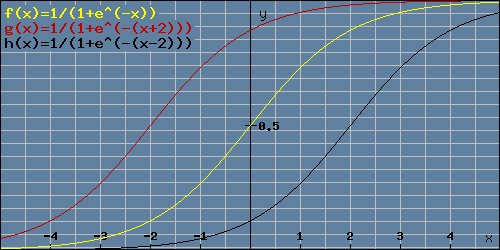
\includegraphics[scale=0.60]{./Images/Pasted image 20231005145933.png}
\caption{Sigmoidfunktion mit Bias}
\label{Sigmoid-Funktion mit Bias}
\end{figure}


\begin{itemize}
  \item Dendriten
  \item der Zellkörper
  \item das Axon
\end{itemize}

\begin{lstlisting}[language=Java]
public class NeuralNetwork {
    Layer[] layers;
    double learnRate;    // Initialisierung
    public NeuralNetwork(double learnRate, int... layerSizes) {
        layers = new Layer[layerSizes.length - 1];
        for (int i = 0; i < layers.length; i++) {
            layers[i] = new Layer(layerSizes[i], layerSizes[i + 1]);
        }
        this.learnRate = learnRate;
    }
}
\end{lstlisting}

Aber verfolgen wir diesen Gedanken doch einmal an einem Beispiel:
Sei $f(w)$ unsere Funktion: $$f(w)=w^2+3$$
Wir nennen die kleine Verschiebung von $w$ jetzt $h$.
Dann gilt zumindest schon einmal: $$\Delta w=(w+h)-w$$Und gekürzt:$$\Delta w=h$$
Dann wäre die Änderungsrate also:$$\ddot{A}nderungsrate = \frac{\Delta e}{\Delta w}$$ $$\frac{\Delta e}{\Delta w}=\frac{f(w+h)-f(w)}{h}$$
Wenn wir uns dann die Mühe machen, $f(w)$ aus zuschreiben, ergibt sich daraus:
$$\frac{\Delta e}{\Delta w}=\frac{(w+h)^2+3-(w^2+3)}{h}$$
Dann fangen wir an Klammern auszurechnen:
$$\frac{\Delta e}{\Delta w}=\frac{w^2+w*h+w*h+h^2+3-w^2-3}{h}$$
$$\frac{\Delta e}{\Delta w}=\frac{w^2+w*h+w*h+h^2-w^2}{h}$$
$$\frac{\Delta e}{\Delta w}=\frac{w*h+w*h+h^2}{h}$$
$h$ kürzen:
$$\frac{\Delta e}{\Delta w}=w+w+h$$
$$\frac{\Delta e}{\Delta w}=2w+h$$Und jetzt zum Interessanten Teil. Da wir $h$ nicht gleich 0 setzten können, können wir allerdings $h$ gegen 0 laufen lassen, dann verwenden wir die Leibniz-Notation. Das bedeutet, dass wir anstatt  $\Delta w$ und  $\Delta e$, wobei $\Delta$ eine sehr kleine Vergrößerung darstellt, jetzt $dw$ und $de$ verwenden, wobei $d$ für eine unendlich kleine Vergrößerung steht, eine sogenannte Infinitesimalzahl.
Das sieht dann ungefähr so aus:
$$\frac{de}{dw}=\lim_{h\to 0} 2w +h$$
$$\frac{de}{dw}=2w$$








\section{Einleitung}
\subsection{Motivation}
Neuronale Netzwerke werden vor allem für Klassifikationsverfahren verwendet. In der Praxis gibt es viele Anwendungsbereiche, in denen es vorteilhaft ist, große Mengen von Daten automatisch zu klassifizieren. Einige Beispiele, wären die Bild- und Schrifterkennung, die man dazu verwendet, Kennschilder von Autos, maschinell auszulesen. Solche Technologien werden immer häufiger auf Parkplätzen und Autobahnen eingesetzt. Aber, auch fast jedes Handy kann mittlerweile Schrift erkennen, die mit der Kamera aufgenommen wird. Auch in der Medizin, beim Auswerten von Röntgenbildern, in der Biologie, zum Erkennen von Pflanzen auf Fotos und noch vielem mehr, werden Neuronale Netzwerke inzwischen eingesetzt.\\
Es gibt kaum einen Bereich, in dem sich nicht eine mögliche Anwendung für Neuronale Netzwerke finden lässt. Ganz besonders aufwändige Netzwerke, werden mittlerweile auch für konstruktive Aufgaben verwendet, wie zum Beispiel Sprachmodelle, unter anderem ChatGPT und Bilder generierende KIs, wie Midjourney.
Typische Probleme, bei welchen neuronale Netzwerke eingesetzt werden, sind komplexe Aufgaben, mit gigantischen Datenmengen.\\
Eine Aufgabe ist zu komplex, wenn eine Lösung nicht manuell programmiert werden kann, unter anderem, bei der Bilderkennung. Außerdem sollten solche Probleme automatisiert werden, weil es sich nicht lohnt, Menschen dazu einzusetzen. 
In solchen Fällen, werden neuronale Netzwerke eingesetzt.\\
Im Laufe der Zeit sind die modernen Netzwerke immer komplexer geworden und liefern nahezu menschliche Ergebnisse, im Bruchteil der Zeit, die Menschen dafür brauchen würden. Aber wie genau funktioniert so ein Netzwerk?



\cleardoublepage
% \phantomsection
\sloppy
\section{Quellen}
\begin{itemize}
\item 1. Alexey Kravets, "Forward and Backward propagation of Max Pooling Layer in Convolutional Neural Networks", URL: https://towardsdatascience.com/forward-and-backward-propagation-of-pooling-layers-in-convolutional-neural-networks-11e36d169bec


\item 2. T. Rashid, Neuronale Netze selbst programmieren - Ein verständlicher Einstieg mit Python. Paderborn: O’Reilly Verlag; 2017.
\item 3. S. Lague, How to Create a Neural Network (and Train it to Identify Doodles). Hrsg. auf dem YouTube Kanal [Sebastian Lague](\url{https://www.youtube.com/@SebastianLague}). Ohne Jahr [zitiert am 16. September 2023]. Abrufbar unter: URL: \url{https://www.youtube.com/watch?v=hfMk-kjRv4c}.
\item 4. "Ableitung der Sigmoid-Funktion" URL: \url{https://ichi.pro/de/ableitung-der-sigmoid-funktion-91708302791054}
\item 5. "What is the role of the bias in neural networks?" URL: \url{https://stackoverflow.com/questions/2480650/what-is-the-role-of-the-bias-in-neural-networks}.
\item 6. "How do I choose the optimal batch size?", URL: \url{https://ai.stackexchange.com/questions/8560/how-do-i-choose-the-optimal-batch-size}
\end{itemize}

\cleardoublepage
\section{Liste der Abbildungen}
\listoffigures
\end{document}